\documentclass[12pt,a4paper]{article}
\usepackage[utf8]{inputenc}
\usepackage[english]{babel}
\usepackage{listings}
\usepackage{xcolor}
\usepackage{graphicx}
\usepackage{geometry}
 \geometry{
 a4paper,
 total={170mm,257mm},
 left=25mm,
 top=20mm,
 right=25mm,
 bottom=20mm
 }

\title{\bf 8 Bit Arithmetic Operations using 8051}
\author{\vspace{-10ex}}
\date{\vspace{-10ex}}
\begin{document}
\maketitle

\begin{minipage}{0.45\textwidth}
        \begin{tabular}{l l}
            \textbf{Expt No:}&12\\
            \textbf{Date :}&23/10/2020
        \end{tabular}
\end{minipage}%
\begin{minipage}{0.45\textwidth}
        \begin{tabular}{l l}
             \textbf{Name:}& Shivanirudh S G  \\
             \textbf{Reg No:} & 185001146 
        \end{tabular}
\end{minipage}
\vspace{1cm}
\hrule
\begin{flushleft}
\subsection*{\textbf{Aim:}} 
To perform arithmetic operations on two 8 bit numbers using \textbf{8051 microcontroller}.

\subsection*{\textbf{\underline{8 Bit Addition}}}

\subsubsection*{\textbf{Algorithm:}}
\begin{itemize}
    \item Move hex value 00 to register 0. 
    \item Move the value of register 1 to A.
    \item Add value in register 2 to A using ADD A, R2
    \item Using JNC instruction check for carry and if there is no carry, no need to increment R0.
    \item Else, increment R0 by 1. 
    \item The result and carry stored in A and R0 should be moved to R4 and R3 respectively.
\end{itemize}

\newpage
\subsubsection*{\textbf{Program:}}

\begin{table}[htb]
\centering
\resizebox{\columnwidth}{!}{
\begin{tabular}{|l|l|} 
\hline
\textbf{Program}                                                 & \textbf{Comments}                             \\ 
\hline
\hline
mov r0, \#00                                                      & Move hex value 00 to Register 0               \\
\hline
mov a, r1                                                        & Move value in Register 1 to A                 \\
\hline
add a, r2                                                        & A = A + R2                                    \\
\hline
jnc label                                                        & Jump if no carry to label LABEL               \\
\hline
inc r0                                                           & Increment value in R0                         \\
\hline
label:~mov r4, a                                                 & Move result in A to Register 4                \\
\hline
mov 03, r0                                                       & Move carry in R0 to R3                        \\
\hline
here:~sjmp here                                                  & Halt                                          \\
\hline
\end{tabular}
}
\end{table}

\subsubsection*{\textbf{Input and Output:}}
\begin{figure}[h]
    \centering
    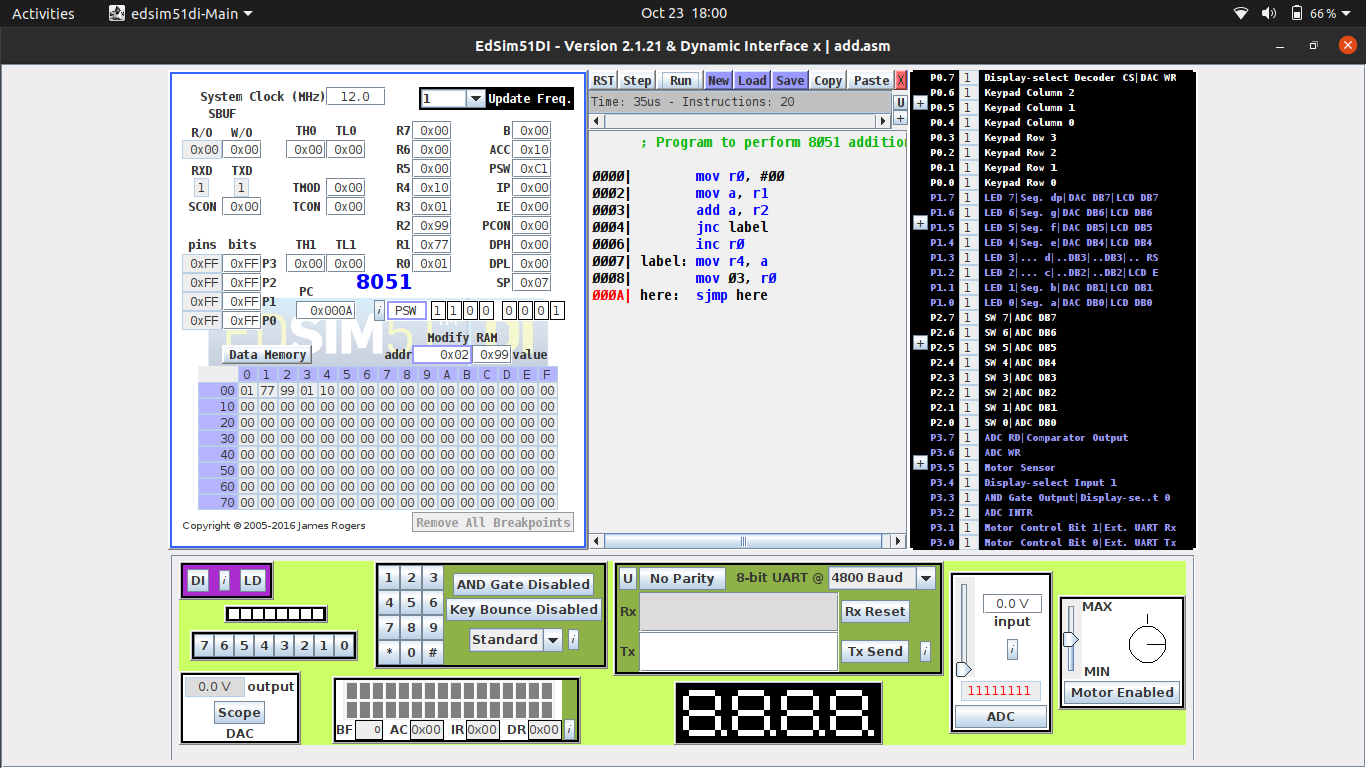
\includegraphics[trim = 60mm 75mm 60mm 10mm, clip, width = \textwidth]{Pics/Add.png}
    \caption{ \textbf{Input:} \emph{r1:} 77h, \emph{r2:} 99h; 
              \textbf{Output:} \emph{Result:} 10h, \emph{Carry:} 01h}
\end{figure}
%----------------------------------------------------------------------------------------------------------------------------------------
\newpage
\subsection*{\textbf{\underline{8 Bit Subtraction}}}

\subsubsection*{\textbf{Algorithm:}}
\begin{itemize}
    \item Move hex value 00 to register 0. 
    \item Move the value of register 1 to A.
    \item Subtract value in register 2 from A using SUBB A, R2
    \item Using JNC instruction check for carry and if there is no carry, no need to increment R0.
    \item Else, increment R0 by 1, complement and increment A by 1. 
    \item The result and sign stored in A and R0 should be moved to R4 and R3 respectively.
\end{itemize}

\newpage
\subsubsection*{\textbf{Program:}}

\begin{table}[htb]
\centering
\resizebox{\columnwidth}{!}{
\begin{tabular}{|l|l|} 
\hline
\textbf{Program}                                                 & \textbf{Comments}                             \\ 
\hline
\hline
mov r0, \#00                                                      & Move hex value 00 to Register 0               \\
\hline
mov a, r1                                                        & Move value in Register 1 to A                 \\
\hline
subb a, r2                                                        & A = A - R2                                    \\
\hline
jnc label                                                        & Jump if no carry to label LABEL               \\
\hline
inc r0                                                           & Increment value in R0                         \\
\hline
cpl a                                                            & Complement value in A                         \\
\hline
inc a                                                            & 2's complement of A                           \\
\hline
label:~mov r4, a                                                 & Move result in A to Register 4                \\
\hline
mov 03, r0                                                       & Move carry in R0 to R3                        \\
\hline
here:~sjmp here                                                  & Halt                                          \\
\hline
\end{tabular}
}
\end{table}

\subsubsection*{\textbf{Input and Output:}}
\begin{figure}[h]
    \centering
    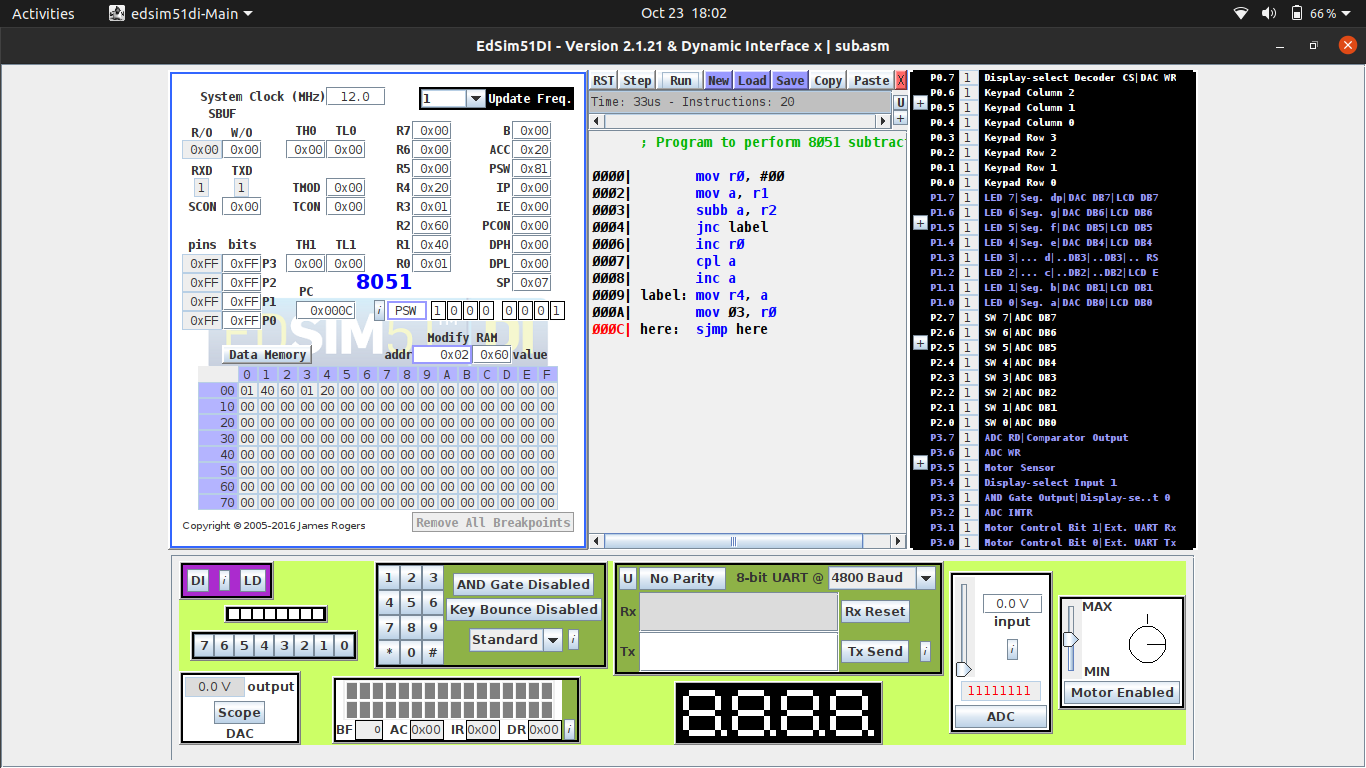
\includegraphics[trim = 60mm 75mm 60mm 10mm, clip, width = \textwidth]{Pics/Sub.png}
    \caption{ \textbf{Input:} \emph{r1:} 40h, \emph{r2:} 60h; 
              \textbf{Output:} \emph{Result:} 20h, \emph{Sign:} 01h}
\end{figure}
\hrule
\subsection*{\textbf{Result:}}
The 8051 programs were written to perform 8-bit arithmetic operations, and the results observed.
\end{flushleft}
\end{document}